\section{ADC}
ADC eller A/D converter er en enhed der benyttes til at omdanne et elektrisk analog signal til et digitalt signal som kan viderebearbejdes i software. 
Den ADC som sidder på PIC32mx250f128b \cite{pic32mx} er en 10 bit ADC, som kan have op til 9 analoge inputs. På UCN boardet er 6 mulige inputs hvoraf gruppen  anvender 3 af disse til lyssensorerne. 

\begin{figure}[h!]
  \centering
  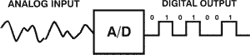
\includegraphics[width=0.7\textwidth]{figures/A_D_converter.png}
  \caption{ADC diagram.\cite{ADC_figur}}
  \label{adcDiagram}
\end{figure} 
\fxnote{fix figur og kilde}
%kilde til http://www.microchip.com/wwwproducts/en/PIC32MX250F128B(hashtag)documents
Den anvendte ADC er implementeret ved hjælp af ADC reference manualen fra microchip, som er et generelt datablad for PIC32 processorene. Her findes de nødvendige opsætninger som skal foretages for at anvende ADC'en efter den ønskede hensigt.
\newline

ADC'en er implementeret ved hjælp af fremgangsmåden anvist i databladet. Her sættes en række registre op efter den ønskede opsætning. 

\begin{figure}[h!]
  \centering
  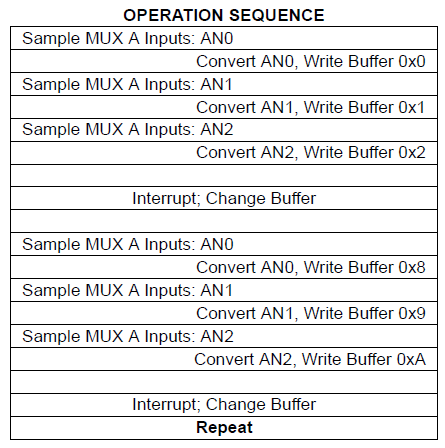
\includegraphics[width=0.7\textwidth]{figures/operation_sequence.png}
  \caption{Operations sekvens.}
  \label{handlingsekvens}
\end{figure} 

Den angivne sekvens viser på figur \ref{handlingsekvens}, hvilken rækkefølge den udfører sine funktioner i. Softwaren gældende for ADC'en er bygget op efter samme princip hvor der først foretages en sampling gennem en positiv målt værdi fra AN0, som er den pin som er tilknyttet vores MUX A(multiplexer). Herfra konverteres den registrerede værdi og tilskriver den digitalt til bufferen. Denne sekvens gør sig gældende for alle 3 sensorer, hvorefter bufferen ændres og et interrupt foretages. 

\begin{figure}[h!]
  \centering
  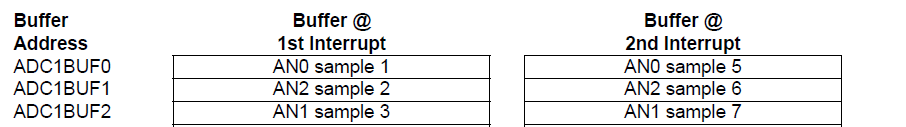
\includegraphics[width=1.1\textwidth]{figures/adcBuffer.png}
  \caption{Tilskrivning til ADC buffer.}\fxnote{kilde til datablad}
  \label{adcBuffer}
\end{figure}

Denne sekvens foretages kontinuerligt af ADC'en, hvor de konverterede målinger skrives til bufferen som vist på figur \ref{adcBuffer}. 

En ADC kan generer noget kaldet "Aliasing" som er kopier af signalet, som bliver genereret ved samplings frekvensen. Dette filtreres væk vha. et low-pass filter\ref{lowPassFilter}.
\newpage
\subsection{ADC deltest}
For at verificere funktionaliteten på ADC'en er en test blevet udført. Testen er udført vha. et FTDI kabel(se figur \ref{ftdi_cable}) som opretter en serial forbindelse på computeren hvor målte ADC værdier kan skrives til. Derved kan det visuelt bekræftes at ADC'en måler en værdi som ligger i indenfor den det forventede område for en 10 bit ADC, som er 1024, eller fra 0 til 1023.


\begin{figure}[h!]
  \centering
  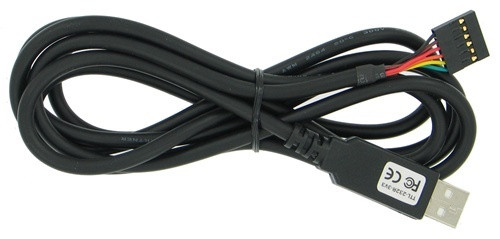
\includegraphics[width=0.5\textwidth]{figures/ftdi_cable.png}
  \caption{ftdi kabel til oprettelse af serial forbindelse.}
  \label{ftdi_cable}
\end{figure} 
Testen blev udført ved at skrive ADC bufferene ud til den serielle port hvor værdierne blev aflæst. Der blev ikke taget højde for hvilke analoge pins der var forbundet til hvad, blot at ADC bufferne blev blev skrevet til den serielle port på PC'en.

\begin{figure}[h!]
  \centering
  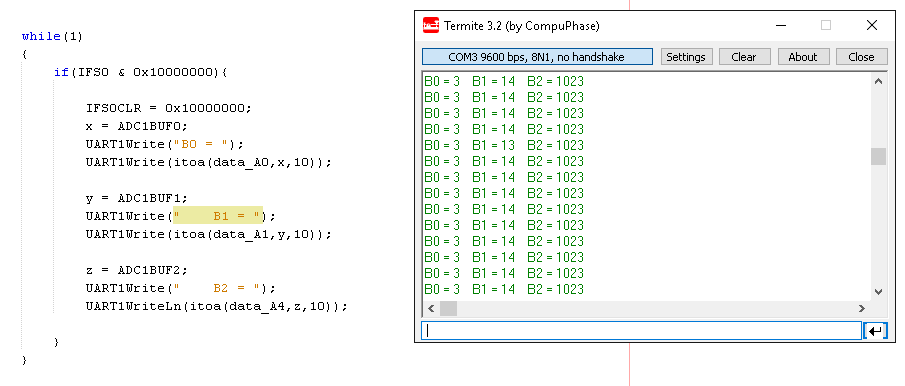
\includegraphics[width=1.0\textwidth]{figures/adc_software_test.png}
  \caption{ADC deltest.}
  \label{adcDelTest}
\end{figure} 


Testen blev foretaget med et potentiometer tilkoblet de 3 ADC indgange (AN3, AN4, AN5) og der blev justeret fra min til maksimum. Det blev observeret at den udskrevne værdi gik fra 0 til 1023, hvilket også er opløsningen på ADC'en. Derved kan det konkluderes at testen var succesfuld for ADC'en.

